\chapter{Teoría de Hückel y sistemas conjugados}\label{ch:b2:huckel}

Al hidrogenar ciclohexeno se liberan \qty{119}{kJ} por mol. El benceno,
con tres dobles enlaces en un anillo de seis carbonos, debería liberar el triple
en su camino hacia el ciclohexano; libera \qty{150}{kJ} menos. Esa energía que
falta es la estabilidad de un anillo \omterm{def:b2:huckel:aromatic}{aromático}, la razón por la que el benceno resiste
las adiciones que sufren los alquenos. En 1931 Erich Hückel la calculó con un
determinante, tras reducir la molécula a sus electrones $\pi$ y a sus
vecinos. Su método es tosco, pero explica por qué los anillos de seis electrones $\pi$
son especiales, por qué las cadenas conjugadas largas absorben luz visible y
dónde lleva sus cargas una molécula conjugada.

\begin{recall}
\Cref{ch:b2:diatomic-mos}: \omterm{def:b2:diatomic-mos:integrals}{integral de Coulomb} $\alpha$, \omterm{def:b2:diatomic-mos:integrals}{integral de resonancia} $\beta$,
\omterm{def:b2:diatomic-mos:integrals}{determinante secular}. \Cref{ch:b2:fragment-orbitals}: orbitales $\pi$ del eteno y del
alilo. El volumen del primer año: sistemas conjugados, resonancia, cromóforos y
máximos de absorción.
\end{recall}

\section{El método de Hückel}

En una molécula conjugada plana, los orbitales $\sigma$ son simétricos y los orbitales p
perpendiculares al plano, antisimétricos respecto de ese plano: no se
mezclan (\cref{prop:b2:diatomic-mos:symmetry}), y los electrones $\pi$ pueden
tratarse por separado.

\begin{definition}[Método de Hückel]\label{def:b2:huckel:method}
El \emph{método de Hückel}\index{metodo de Huckel@método de Hückel} calcula los orbitales $\pi$ de un
sistema conjugado plano como combinaciones $\psi = \sum_r c_r p_r$ de un orbital p por
átomo, con las aproximaciones: solapamientos $S_{rs} = 0$ para $r \neq s$ (y 1 para $r =
s$); \omterm{def:b2:diatomic-mos:integrals}{integrales de Coulomb} todas iguales a $\alpha$; \omterm{def:b2:diatomic-mos:integrals}{integrales de resonancia} iguales a $\beta < 0$
entre vecinos enlazados y nulas en los demás casos.
\end{definition}

Con $x = (\alpha - E)/\beta$, las ecuaciones seculares son, para cada átomo $r$,
$xc_r + \sum_{s \text{ enlazado a } r} c_s = 0$, y las energías son las raíces de un
determinante con $x$ en la diagonal y 1 entre átomos enlazados. De forma equivalente, $E =
\alpha + m\beta$, donde los $m$ son los valores propios de la matriz de adyacencia del
esqueleto carbonado de la molécula; como $\beta < 0$, un $m$ positivo corresponde a un nivel enlazante.

\begin{method}[Un cálculo de Hückel]\label{met:b2:huckel:huckel}
\begin{enumerate}
  \item Numérense los átomos conjugados; escríbase la matriz con 0 en la diagonal y 1
        para cada pareja enlazada.
  \item Búsquense sus valores propios $m_k$ (con las fórmulas cerradas siguientes, o numéricamente): $E_k =
        \alpha + m_k\beta$.
  \item Llénense los niveles empezando por el más enlazante, con dos electrones cada uno:
        $E_\pi = \sum_k n_k E_k$.
  \item A partir de los coeficientes normalizados, calcúlense las cargas y los índices de enlace.
\end{enumerate}
\end{method}

\begin{proposition}[Traza]\label{prop:b2:huckel:trace}
Las energías de los $n$ orbitales $\pi$ de un sistema de Hückel suman $n\alpha$.
\end{proposition}

\begin{proof}
La suma de los valores propios de una matriz es su traza; la matriz de Hückel tiene $\alpha$
en cada uno de sus $n$ elementos diagonales.
\end{proof}

\section{Polienos lineales}

\begin{theorem}[Niveles de una cadena lineal]\label{thm:b2:huckel:polyene}
Una cadena conjugada lineal de $n$ átomos tiene los niveles y los coeficientes
\[
  E_k = \alpha + 2\beta\cos\frac{k\pi}{n + 1}, \qquad
  c_{jk} = \sqrt{\frac{2}{n + 1}}\,\sin\frac{jk\pi}{n + 1}, \qquad k = 1, \dots, n .
\]
\end{theorem}

\begin{proof}
Las ecuaciones seculares son $c_{j-1} + xc_j + c_{j+1} = 0$ para $j = 1, \dots, n$, con
$c_0 = c_{n+1} = 0$. Probemos $c_j = \sin j\theta$: $\sin(j - 1)\theta + \sin(j + 1)\theta = 2\sin
j\theta\cos\theta$, de modo que las ecuaciones se cumplen con $x = -2\cos\theta$, y $c_0 = 0$
automáticamente. La condición en el extremo, $c_{n+1} = \sin(n + 1)\theta = 0$, da $\theta =
k\pi/(n + 1)$. Entonces $E = \alpha - x\beta = \alpha + 2\beta\cos\theta$. La normalización usa
$\sum_{j=1}^n\sin^2 j\theta = (n + 1)/2$.
\end{proof}

\begin{example}[El butadieno]\label{ex:b2:huckel:butadiene}
Para $n = 4$: $E = \alpha \pm 1.618\beta$, $\alpha \pm 0.618\beta$. Cuatro electrones $\pi$ llenan los dos
niveles enlazantes: $E_\pi = 4\alpha + 2(1.618 + 0.618)\beta = 4\alpha + 4.472\beta$. El orbital
más bajo tiene los coeficientes 0.372, 0.602, 0.602, 0.372, y el siguiente, 0.602, 0.372,
$-0.372$, $-0.602$.
\end{example}

\begin{omfigure}
\begin{tikzpicture}[font=\small]
  \foreach \k/\a/\b/\c/\d/\lab in {1/0.372/0.602/0.602/0.372/{$\psi_1$, $\alpha + 1.618\beta$},
      2/0.602/0.372/-0.372/-0.602/{$\psi_2$, $\alpha + 0.618\beta$},
      3/0.602/-0.372/-0.372/0.602/{$\psi_3$, $\alpha - 0.618\beta$},
      4/0.372/-0.602/0.602/-0.372/{$\psi_4$, $\alpha - 1.618\beta$}} {
    \begin{scope}[yshift={(\k-1)*2.1cm}]
      \draw[black!40] (-0.2,0) -- (3.2,0);
      \pic at (0,0) {omp={1.6*\a}{90}}; \pic at (1,0) {omp={1.6*\b}{90}};
      \pic at (2,0) {omp={1.6*\c}{90}}; \pic at (3,0) {omp={1.6*\d}{90}};
      \node[anchor=west] at (3.6,0) {\lab};
    \end{scope}
  }
\end{tikzpicture}

{\small Los cuatro orbitales $\pi$ del butadieno, con los lóbulos dibujados en proporción a los
coeficientes de Hückel (calculados) y coloreados según su signo; las energías crecen
hacia arriba, con $0, 1, 2, 3$ nodos. Los dos orbitales inferiores están llenos.}
\end{omfigure}

\begin{definition}[Cargas $\pi$ e índices de enlace]\label{def:b2:huckel:indices}
Con $n_k$ electrones en el orbital $k$ (0, 1 o 2) y coeficientes reales $c_{rk}$, la
\emph{carga $\pi$}\index{carga pi@carga $\pi$} sobre el átomo $r$ es $q_r = \sum_k n_kc_{rk}^2$ (el
número de electrones $\pi$ que lleva), y el \emph{índice de enlace $\pi$}\index{indice de enlace pi@índice de enlace $\pi$}
del enlace $rs$ es $p_{rs} = \sum_k n_kc_{rk}c_{sk}$.
\end{definition}

Para el butadieno, $p_{12} = 2(0.372 \times 0.602 + 0.602 \times 0.372) = 0.894$ y $p_{23} =
2(0.602^2 - 0.372^2) = 0.447$: los enlaces de los extremos llevan la mayor parte del enlace $\pi$ y son
los más cortos, y el enlace central tiene un carácter parcial de doble enlace. Todas las cargas valen
1.

\begin{proposition}[Hidrocarburos alternantes]\label{prop:b2:huckel:alternant}
En un hidrocarburo neutro cuyos átomos conjugados pueden colorearse en dos conjuntos sin
que dos vecinos pertenezcan al mismo conjunto (sin anillos impares), todas las cargas $\pi$ valen 1.
\end{proposition}

\admitted

El resultado (de Coulson y Rushbrooke) se comprueba más arriba en el butadieno y, en el benceno, por
simetría; es la razón por la que estos hidrocarburos no tienen dipolo permanente debido a sus
electrones $\pi$.

\begin{definition}[Energía de deslocalización]\label{def:b2:huckel:delocalisation}
La \emph{energía de deslocalización}\index{energia de deslocalizacion@energía de deslocalización} de un sistema
conjugado es la diferencia entre su energía $\pi$ y la del mismo número de
dobles enlaces aislados, cada uno con $E_\pi = 2\alpha + 2\beta$.
\end{definition}

Para el butadieno vale $4.472\beta - 4\beta = 0.472\beta$; para el hexatrieno, $0.988\beta$.

\section{Anillos y aromaticidad}

\begin{theorem}[Niveles de un anillo]\label{thm:b2:huckel:ring}
Un anillo plano de $n$ átomos conjugados tiene los niveles $E_k = \alpha + 2\beta\cos(2\pi k/n)$,
$k = 0, 1, \dots, n - 1$: un nivel más bajo $\alpha + 2\beta$, luego parejas de niveles
degenerados y, para $n$ par, un nivel más alto $\alpha - 2\beta$.
\end{theorem}

\begin{proof}
En un anillo cada átomo tiene dos vecinos, con índices tomados módulo $n$:
$c_{j-1} + xc_j + c_{j+1} = 0$ para todo $j$ y $c_{j+n} = c_j$. Probemos $c_j = \mathrm e^{\mathrm
i jq}$: la ecuación da $x = -(\mathrm e^{-\mathrm iq} + \mathrm e^{\mathrm iq}) = -2\cos q$,
y la periodicidad exige $nq = 2\pi k$. Los niveles $k$ y $n - k$ tienen la misma
energía; su suma y su diferencia son orbitales reales. Solo $k = 0$ (y $k = n/2$ para
$n$ par) es simple.
\end{proof}

\begin{corollary}[El círculo de Frost]\label{cor:b2:huckel:frost}
Los niveles de un anillo se leen en un círculo de radio $2|\beta|$ centrado en $\alpha$, en
el que se inscribe un $n$-ágono regular con un vértice abajo: cada vértice está
a la altura de un nivel.
\end{corollary}

\begin{proof}
El vértice $k$ del polígono se encuentra en el ángulo $-\pi/2 + 2\pi k/n$, y su altura respecto del centro es
$-2|\beta|\cos(2\pi k/n) = 2\beta\cos(2\pi k/n)$.
\end{proof}

\begin{omfigure}
\begin{tikzpicture}[font=\scriptsize]
  \foreach \n/\x/\name/\el in {4/0/{\ce{C4H4}}/4, 5/3.4/{\ce{C5H5-}}/6, 6/6.8/{\ce{C6H6}}/6, 7/10.2/{\ce{C7H7+}}/6} {
    \begin{scope}[xshift=\x cm]
      \draw[black!35] (0,0) circle (1.2);
      \draw[black!60] \foreach \k in {0,...,\the\numexpr\n-1\relax} { ({-90+360*\k/\n}:1.2) -- ({-90+360*(\k+1)/\n}:1.2) };
      \foreach \k in {0,...,\the\numexpr\n-1\relax} {
        \draw[very thick] ({1.2*cos(-90+360*\k/\n)-0.22},{1.2*sin(-90+360*\k/\n)}) -- ({1.2*cos(-90+360*\k/\n)+0.22},{1.2*sin(-90+360*\k/\n)});
      }
      \draw[densely dotted] (-1.5,0) -- (1.5,0);
      \node[font=\small] at (0,-1.75) {\name};
    \end{scope}
  }
  \node[anchor=east] at (-1.5,0) {$\alpha$};
  % electrons: C4H4 (2 + 1 + 1), others filled lowest three
  \foreach \x in {0,3.4,6.8,10.2} {
    \draw[-{Stealth[length=1mm]}, thick] ({\x-0.05},-1.32) -- ({\x-0.05},-1.08);
    \draw[-{Stealth[length=1mm]}, thick] ({\x+0.05},-1.08) -- ({\x+0.05},-1.32);
  }
  % six-electron rings: the lowest degenerate pair is filled
  \foreach \n/\x in {5/3.4, 6/6.8, 7/10.2} {
    \foreach \k in {1, \the\numexpr\n-1\relax} {
      \pgfmathsetmacro\ex{\x + 1.2*cos(-90 + 360*\k/\n)}
      \pgfmathsetmacro\ey{1.2*sin(-90 + 360*\k/\n)}
      \draw[-{Stealth[length=1mm]}, thick] ({\ex-0.05},{\ey-0.12}) -- ({\ex-0.05},{\ey+0.12});
      \draw[-{Stealth[length=1mm]}, thick] ({\ex+0.05},{\ey+0.12}) -- ({\ex+0.05},{\ey-0.12});
    }
  }
  % C4H4: one electron in each of the two nonbonding levels
  \draw[-{Stealth[length=1mm]}, thick] (1.2,-0.12) -- (1.2,0.12);
  \draw[-{Stealth[length=1mm]}, thick] (-1.2,-0.12) -- (-1.2,0.12);
\end{tikzpicture}

{\small Círculos de Frost. Los vértices de cada polígono, inscrito con un vértice
abajo en un círculo de radio $2|\beta|$, dan los niveles del anillo. Con seis electrones
$\pi$, \ce{C5H5-}, \ce{C6H6} y \ce{C7H7+} llenan el nivel más bajo y una pareja
degenerada: capas cerradas. Los cuatro electrones del ciclobutadieno dejan dos electrones en una
pareja degenerada no enlazante (dibujados).}
\end{omfigure}

\begin{definition}[Aromaticidad]\label{def:b2:huckel:aromatic}
Un sistema cíclico, plano y totalmente conjugado es \emph{aromático}\index{aromatico@aromático} cuando
sus electrones $\pi$ forman una capa cerrada con una gran \omterm{def:b2:huckel:delocalisation}{energía de deslocalización}, y
\emph{antiaromático}\index{antiaromatico@antiaromático} cuando sus electrones $\pi$ llenan a medias una pareja
degenerada, lo que lo hace menos estable que la cadena abierta correspondiente.
\end{definition}

\begin{theorem}[Regla de Hückel]\label{thm:b2:huckel:huckel-rule}
Un sistema conjugado monocíclico plano tiene una capa cerrada de electrones $\pi$ si y solo
si contiene $4N + 2$ de ellos ($N = 0, 1, 2, \dots$); con $4N$ tiene dos electrones en una
pareja degenerada llena a medias. Es la \emph{regla de Hückel}\index{regla de Huckel@regla de Hückel}.
\end{theorem}

\begin{proof}
Por el \cref{thm:b2:huckel:ring}, los niveles desde abajo son un nivel simple y
luego parejas degeneradas (en la parte ocupada). Una capa cerrada llena el nivel
simple (2 electrones) y un número entero $N$ de parejas (4 electrones cada una): $4N + 2$. Con
$4N$ electrones, la última pareja solo contiene dos, uno en cada uno de sus orbitales (regla de
Hund).
\end{proof}

\begin{method}[¿Es aromático?]\label{met:b2:huckel:aromaticity}
\begin{enumerate}
  \item ¿Es el sistema un anillo con un orbital p en cada átomo (contando los centros
        carbocatiónicos y carbaniónicos y los pares no enlazantes de los heteroátomos)?
  \item ¿Puede ser plano?
  \item Cuéntense los electrones $\pi$: $4N + 2$, \omterm{def:b2:huckel:aromatic}{aromático}; $4N$, \omterm{def:b2:huckel:aromatic}{antiaromático} si es plano.
  \item Un anillo \omterm{def:b2:huckel:aromatic}{antiaromático} evita la planaridad o la conjugación cuando puede
        (el ciclooctatetraeno tiene forma de bañera y se comporta como un polieno).
\end{enumerate}
\end{method}

\begin{example}[El benceno]\label{ex:b2:huckel:benzene}
Seis electrones $\pi$ llenan $\alpha + 2\beta$ y la pareja $\alpha + \beta$: $E_\pi = 6\alpha + 8\beta$.
Tres dobles enlaces aislados dan $6\alpha + 6\beta$: la \omterm{def:b2:huckel:delocalisation}{energía de deslocalización} es $2\beta$,
aproximadamente el doble que la de la cadena abierta de seis carbonos, el hexatrieno ($0.988\beta$): cerrar
el anillo vale otro tanto. Por simetría, todos los índices de enlace son iguales ($p = 2/3$), y también lo son las seis
longitudes de enlace, \qty{139.7}{pm}, entre las del eteno (\qty{133.9}{pm}) y el etano
(\qty{153.6}{pm}).
% ledger: geo:C6H6.rCC, geo:C2H4.rCC, geo:C2H6.rCC
\end{example}

\begin{omfigure}
\begin{tikzpicture}[font=\small, y=0.013cm, x=1.0cm]
  \draw[thick] (0,0) -- (10.5,0);
  \node[anchor=north] at (5.2,-8) {ciclohexano (referencia $\Delta_r H = 0$)};
  % cyclohexene
  \draw[thick, omDef] (0.6,118.8) -- (1.6,118.8); \draw[->, omDef] (1.1,118.8) -- (1.1,4);
  \node[font=\scriptsize, anchor=south, align=center] at (1.1,120) {ciclohexeno\\ \qty{118.8}{kJ/mol}};
  % diene
  \draw[thick, omDef] (3.6,227.7) -- (4.6,227.7); \draw[->, omDef] (4.1,227.7) -- (4.1,4);
  \draw[thick, black!45, densely dashed] (4.7,237.6) -- (5.6,237.6);
  \node[font=\scriptsize, anchor=south, black!60] at (5.15,240) {$2 \times 118.8$};
  \node[font=\scriptsize, anchor=east, align=right] at (3.5,227.7) {ciclohexa-1,3-dieno\\ \qty{227.7}{kJ/mol}};
  % benzene
  \draw[thick, omDef] (7.6,206.0) -- (8.6,206.0); \draw[->, omDef] (8.1,206.0) -- (8.1,4);
  \node[font=\scriptsize, anchor=east, align=right] at (7.5,206.0) {benceno\\ \qty{206.0}{kJ/mol}};
  \draw[thick, black!45, densely dashed] (7.6,356.4) -- (8.6,356.4);
  \node[font=\scriptsize, anchor=south, black!60] at (8.1,358) {$3 \times 118.8 = 356.4$};
  \draw[<->, omThm, thick] (8.9,206) -- (8.9,356.4) node[midway, right, font=\scriptsize] {\qty{150}{kJ/mol}};
\end{tikzpicture}

{\small Entalpías de hidrogenación a ciclohexano en fase gaseosa, a partir de entalpías de
formación tabuladas (barras, altura = calor liberado). Dos dobles enlaces conjugados
liberan \qty{10}{kJ/mol} menos que el doble de uno; el benceno libera \qty{150}{kJ/mol} menos que
el triple de uno: su estabilización \omterm{def:b2:huckel:aromatic}{aromática}.}
% ledger: dfh:C6H6_g, dfh:C6H10_g, dfh:C6H12_g, dfh:C6H8_g
\end{omfigure}

\begin{history}[El anillo de Kekulé]
\begin{minipage}[t]{0.22\linewidth}
\vspace{0pt}
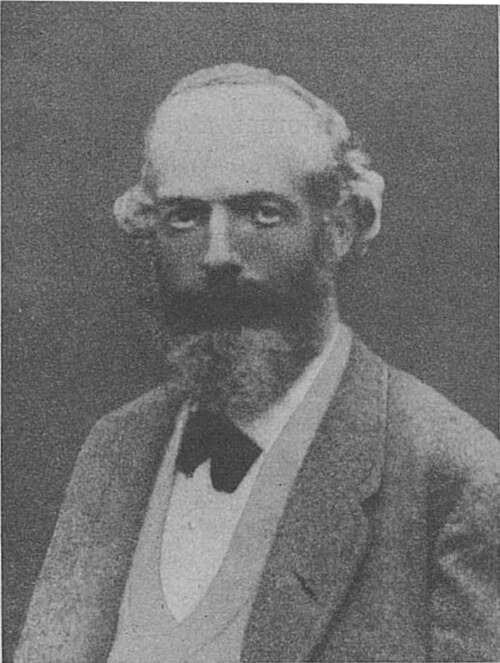
\includegraphics[width=\linewidth]{images/book3/kekule.jpg}
\end{minipage}\hfill
\begin{minipage}[t]{0.74\linewidth}
\vspace{0pt}
En 1865 August Kekulé propuso que los seis átomos de carbono del benceno forman un anillo
con enlaces sencillos y dobles alternos, y poco después, que las dos alternancias
se intercambian tan deprisa que todos los enlaces son iguales. Los enlaces iguales hallados por difracción
de rayos X, y los orbitales $\pi$ extendidos por todo el anillo, dieron a su intuición su
forma moderna; la \omterm{thm:b2:huckel:huckel-rule}{regla de Hückel}, en 1931, explicó por qué seis electrones, y no cuatro u
ocho, hacen especial un anillo. (Retrato, 1873, autor desconocido, dominio público,
Wikimedia Commons.)
\end{minipage}
\end{history}

\section{Conjugación y luz}

\begin{proposition}[La diferencia de energía de un polieno]\label{prop:b2:huckel:gap}
En un polieno lineal de $n$ carbonos ($n$ par), la diferencia entre el nivel $\pi$ ocupado más alto
y el vacío más bajo es $4|\beta|\sin(\pi/(2(n + 1)))$: disminuye a medida que la
cadena se alarga.
\end{proposition}

\begin{proof}
El nivel ocupado más alto es $k = n/2$, y el vacío más bajo, $k = n/2 + 1$. Con $\theta_k =
k\pi/(n + 1)$, $E_{n/2+1} - E_{n/2} = 2|\beta|(\cos\theta_{n/2} - \cos\theta_{n/2+1}) = 4|\beta|
\sin\frac{\theta_{n/2} + \theta_{n/2+1}}{2}\sin\frac{\theta_{n/2+1} - \theta_{n/2}}{2}$, y el
primer seno es $\sin(\pi/2) = 1$. Disminuye con $n$ porque $\sin$ es creciente en
$[0, \pi/2]$.
\end{proof}

\begin{omfigure}
\begin{tikzpicture}
\begin{axis}[width=0.5\linewidth, height=5cm, xmin=0, xmax=22, ymin=0, ymax=2.2,
  axis x line=bottom, axis y line=left, xlabel={carbonos $n$}, ylabel={diferencia$/|\beta|$},
  tick label style={font=\small}, label style={font=\small}]
\addplot[omThm, thick, mark=*, mark size=1.3pt] table[x=n, y=gap] {figdata/out/bachelor-2-huckel-b.dat};
\end{axis}
\end{tikzpicture}\hfill
\begin{tikzpicture}
\begin{axis}[width=0.48\linewidth, height=5.4cm, xmin=-1, xmax=11, ymin=-2.4, ymax=2.4,
  axis x line=none, axis y line=left, ylabel={$(E - \alpha)/|\beta|$}, clip=false,
  tick label style={font=\small}, label style={font=\small}]
\addplot[only marks, mark=-, mark size=5pt, very thick, omDef] table[x=x, y=e] {figdata/out/bachelor-2-huckel-a.dat};
\draw[densely dotted] (axis cs:-1,0) -- (axis cs:11,0);
\node[anchor=north, font=\scriptsize] at (axis cs:0,-2.45) {C$_2$};
\node[anchor=north, font=\scriptsize] at (axis cs:2,-2.45) {C$_3$};
\node[anchor=north, font=\scriptsize] at (axis cs:4,-2.45) {C$_4$};
\node[anchor=north, font=\scriptsize] at (axis cs:6,-2.45) {C$_6$};
\node[anchor=north, font=\scriptsize] at (axis cs:8,-2.45) {anillo 4};
\node[anchor=north, font=\scriptsize] at (axis cs:10,-2.45) {anillo 6};
\end{axis}
\end{tikzpicture}

{\small A la izquierda: la diferencia de Hückel de los polienos lineales disminuye a medida que crece la cadena,
la razón por la que las cadenas conjugadas largas absorben a longitudes de onda mayores, hasta el visible.
A la derecha: niveles calculados del eteno, el alilo, el butadieno y el hexatrieno (cadenas) y del
ciclobutadieno y el benceno (anillos); los niveles enlazantes, por debajo de $\alpha$.}
\end{omfigure}

Un heteroátomo se introduce cambiando su \omterm{def:b2:diatomic-mos:integrals}{integral de Coulomb}, $\alpha_X = \alpha + h\beta$, y las
\omterm{def:b2:diatomic-mos:integrals}{integrales de resonancia} de sus enlaces: un modelo con parámetros ajustables, que conserva los
resultados cualitativos (un átomo electronegativo, $h > 0$, atrae hacia sí la densidad $\pi$)
pero cuyos números se ajustan, no se deducen.

\section{Ejercicios}

\begin{exercise}[$\star$]\label{exo:b2:huckel:1}
Dese $E_\pi$ para el catión, el radical y el anión alilo.
\end{exercise}

\begin{exercise}[$\star$]\label{exo:b2:huckel:2}
Calcúlese la $E_\pi$ del butadieno a partir de los niveles $\alpha \pm 1.618\beta$, $\alpha \pm 0.618\beta$.
\end{exercise}

\begin{exercise}[$\star$]\label{exo:b2:huckel:3}
¿\omterm{def:b2:huckel:aromatic}{Aromático}, \omterm{def:b2:huckel:aromatic}{antiaromático} o ninguno de los dos (si es plano)?: benceno, anión ciclopentadienilo,
catión ciclopentadienilo, catión tropilio \ce{C7H7+}, ciclobutadieno y
ciclooctatetraeno plano.
\end{exercise}

\begin{exercise}[$\star$]\label{exo:b2:huckel:4}
Dibújese el círculo de Frost del ciclooctatetraeno plano y sitúense sus ocho electrones $\pi$.
\end{exercise}

\begin{exercise}[$\star\star$]\label{exo:b2:huckel:5}
Calcúlese la \omterm{def:b2:huckel:delocalisation}{energía de deslocalización} del butadieno y dese en \unit{kJ/mol} con
$|\beta| = \qty{75}{kJ/mol}$. Compárese con los \qty{10}{kJ/mol} de los datos de hidrogenación
del ciclohexa-1,3-dieno.
\end{exercise}

\begin{exercise}[$\star\star$]\label{exo:b2:huckel:6}
Calcúlense los índices de enlace $\pi$ del butadieno y prevéase cuál de sus enlaces C--C es el
más corto.
\end{exercise}

\begin{exercise}[$\star\star$]\label{exo:b2:huckel:7}
Los niveles de un anillo de cinco eslabones son $\alpha + 2\beta$, $\alpha + 0.618\beta$ (dos veces),
$\alpha - 1.618\beta$ (dos veces). Llénense para el anión y el catión ciclopentadienilo y
compárense.
\end{exercise}

\begin{exercise}[$\star\star$]\label{exo:b2:huckel:8}
Con los niveles de un anillo de siete eslabones, explíquese por qué el bromuro de cicloheptatrienilo
se comporta como una sal, el bromuro de tropilio.
\end{exercise}

\begin{exercise}[$\star\star$]\label{exo:b2:huckel:9}
Compruébese la regla de la traza en el hexatrieno, cuyos niveles son $\alpha \pm 1.802\beta$, $\alpha \pm
1.247\beta$, $\alpha \pm 0.445\beta$.
\end{exercise}

\begin{exercise}[$\star\star\star$]\label{exo:b2:huckel:10}
Dedúzcanse los niveles del hexatrieno a partir de la fórmula cerrada, y su \omterm{def:b2:huckel:delocalisation}{energía de deslocalización}.
\end{exercise}

\begin{exercise}[$\star\star\star$]\label{exo:b2:huckel:11}
El ciclobutadieno cuadrado tendría dos electrones desapareados. Explíquese por qué la molécula real
es rectangular, con dos enlaces cortos y dos largos.
\end{exercise}

\begin{exercise}[$\star\star\star$]\label{exo:b2:huckel:12}
En un sistema $\pi$ de dos átomos \ce{C=X} con $\alpha_X = \alpha + \beta$ (valor del modelo, $h = 1$) y
$\beta_{\ce{CX}} = \beta$, hállense los dos niveles y las cargas $\pi$ sobre C y X para dos
electrones.
\end{exercise}

\section{Problema: la energía que le falta al benceno}

\begin{problem}[{Problema de fin de semana --- la estabilización aromática del benceno a partir de
las entalpías de hidrogenación, los niveles de Hückel del benceno y su energía de
deslocalización, el valor de $|\beta|$ y la comparación con el hexatrieno y el
ciclooctatetraeno}]
\label{pb:b2:huckel:1}
Datos: entalpías de formación de los gases (\unit{kJ/mol}): benceno 82.9,
ciclohexa-1,3-dieno 104.6, ciclohexeno $-4.3$, ciclohexano $-123.1$. Longitudes de enlace
(pm): benceno 139.7, eteno 133.9, etano 153.6.
% ledger: dfh:C6H6_g, dfh:C6H8_g, dfh:C6H10_g, dfh:C6H12_g, geo:C6H6.rCC, geo:C2H4.rCC, geo:C2H6.rCC

\medskip
\noindent\textbf{Parte I --- Hidrogenación.}
\begin{enumerate}
  \item Calcúlese el $\Delta_r H^\circ$ de la hidrogenación del ciclohexeno a ciclohexano.
  \item Lo mismo para el ciclohexa-1,3-dieno.
  \item Lo mismo para el benceno.
  \item ¿Qué liberarían tres dobles enlaces independientes?
  \item Dedúzcase la estabilización del benceno.
  \item Compárese con la del dieno conjugado, y coméntese.
\end{enumerate}

\medskip
\noindent\textbf{Parte II --- El benceno según Hückel.}
\begin{enumerate}[resume]
  \item Escríbase la matriz de Hückel del benceno.
  \item Dense sus niveles a partir de la fórmula del anillo.
  \item Llénense con seis electrones $\pi$.
  \item Calcúlese $E_\pi$.
  \item Calcúlese la $E_\pi$ de tres dobles enlaces aislados.
  \item Dedúzcase la \omterm{def:b2:huckel:delocalisation}{energía de deslocalización}.
  \item Compruébese la regla de la traza.
\end{enumerate}

\medskip
\noindent\textbf{Parte III --- El valor de $|\beta|$.}
\begin{enumerate}[resume]
  \item Iguálese la \omterm{def:b2:huckel:delocalisation}{energía de deslocalización} a la estabilización de la Parte I y hállese
        $|\beta|$.
  \item Con ese valor, prevéase la \omterm{def:b2:huckel:delocalisation}{energía de deslocalización} del butadieno, y compárese
        con la Parte I.
  \item Calcúlense los índices de enlace $\pi$ del benceno.
  \item Compárense con los del butadieno.
  \item Explíquese por qué las longitudes de enlace del benceno son iguales y dónde se sitúan.
\end{enumerate}

\medskip
\noindent\textbf{Parte IV --- Otros anillos y cadenas.}
\begin{enumerate}[resume]
  \item Calcúlese la \omterm{def:b2:huckel:delocalisation}{energía de deslocalización} del hexatrieno y compárese con el benceno.
  \item Dense los niveles del ciclooctatetraeno plano.
  \item Llénense con ocho electrones: ¿qué falla?
  \item ¿Cómo escapa la molécula real?
  \item ¿Cuál es la situación del ciclobutadieno?
  \item Enúnciese la \omterm{thm:b2:huckel:huckel-rule}{regla de Hückel}.
  \item Indíquese el valor de $|\beta|$ obtenido igualando la \omterm{def:b2:huckel:delocalisation}{energía de deslocalización} del benceno
        con su estabilización medida.
\end{enumerate}
\end{problem}
